\documentclass{article}
\usepackage{graphicx}
\usepackage{float}
\usepackage{subcaption}
\usepackage{amsmath}
\usepackage[utf8]{inputenc}
\usepackage{listings}
\usepackage{minted}

\begin{document}
\title{ 6.320 Final Project Report \\ 
Using Sate Space Modelling for Self-Standing Robot}
\author{Dimitris Koutentakis}
\date{}
\maketitle


\vspace{5mm}
\textbf{Abstract}
\vspace{2mm}

In the project, we take a look at the classic "inverted pendulum" controls problem, and implementing a working solution on a \texttt{Pololu Balboa} robot platform. We build the robot, design a state-space model and discuss its performance with gains obtained from the $LQR$ method. Our final robot was able to stand for an unlimited amount of time, though stabilization after an external disturbance took time to be achieved.

\section{Introduction}

Controlling an upright two-wheeled robot has been a problem of interest for a long time. Be it for commercial applications such as SEGWAY, or military/medical/anthropomorphic robots, the current setup has received a lot of attention and very effective solutions have been found. Here we discuss an implementation of LQR and manual gain tuning in order to effectively control the robot.
The problem is part of the more general inverted pendulum problem, described in figure \ref{pendulum}.

\begin{figure}[H]
    \caption{Inverted Pendulum}
    \centering
    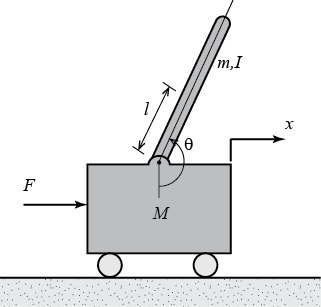
\includegraphics[width=0.6\textwidth]{pendulum.png}
    \label{pendulum}
\end{figure}
    
According to the body diagram of our problem, which is drawn in figure \ref{fbd}, we develop a state-space model and with the help of \texttt{MATLAB} and the LQR method, find appropriate gains for our system.

\begin{figure}[H]
    \caption{Free Body Diagram}
    \centering
    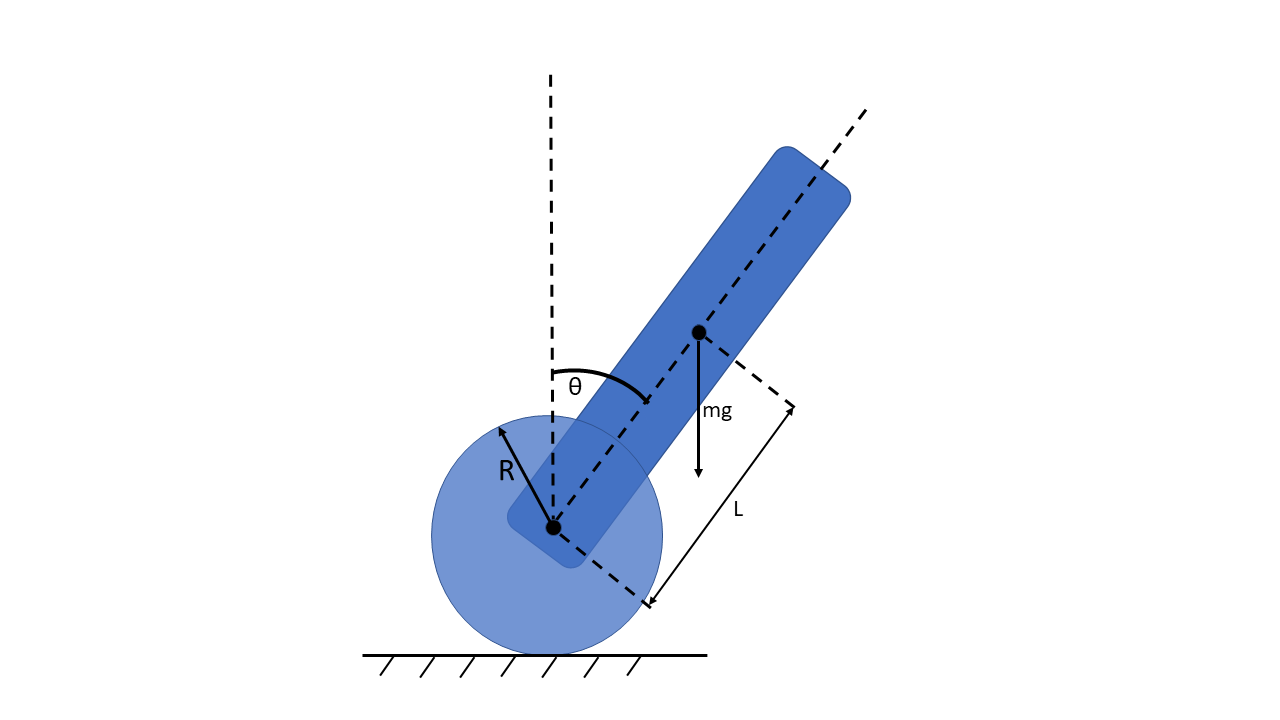
\includegraphics[width=0.75\textwidth]{FBD.png}
    \label{fbd}
\end{figure}
    

\section{Robot}

The robot we used was the Pololu Balboa two-wheel robot shown in Fig. \ref{robot3}. 

\begin{figure}[H]
    \caption{Pololu Balboa Robot}
    \centering
    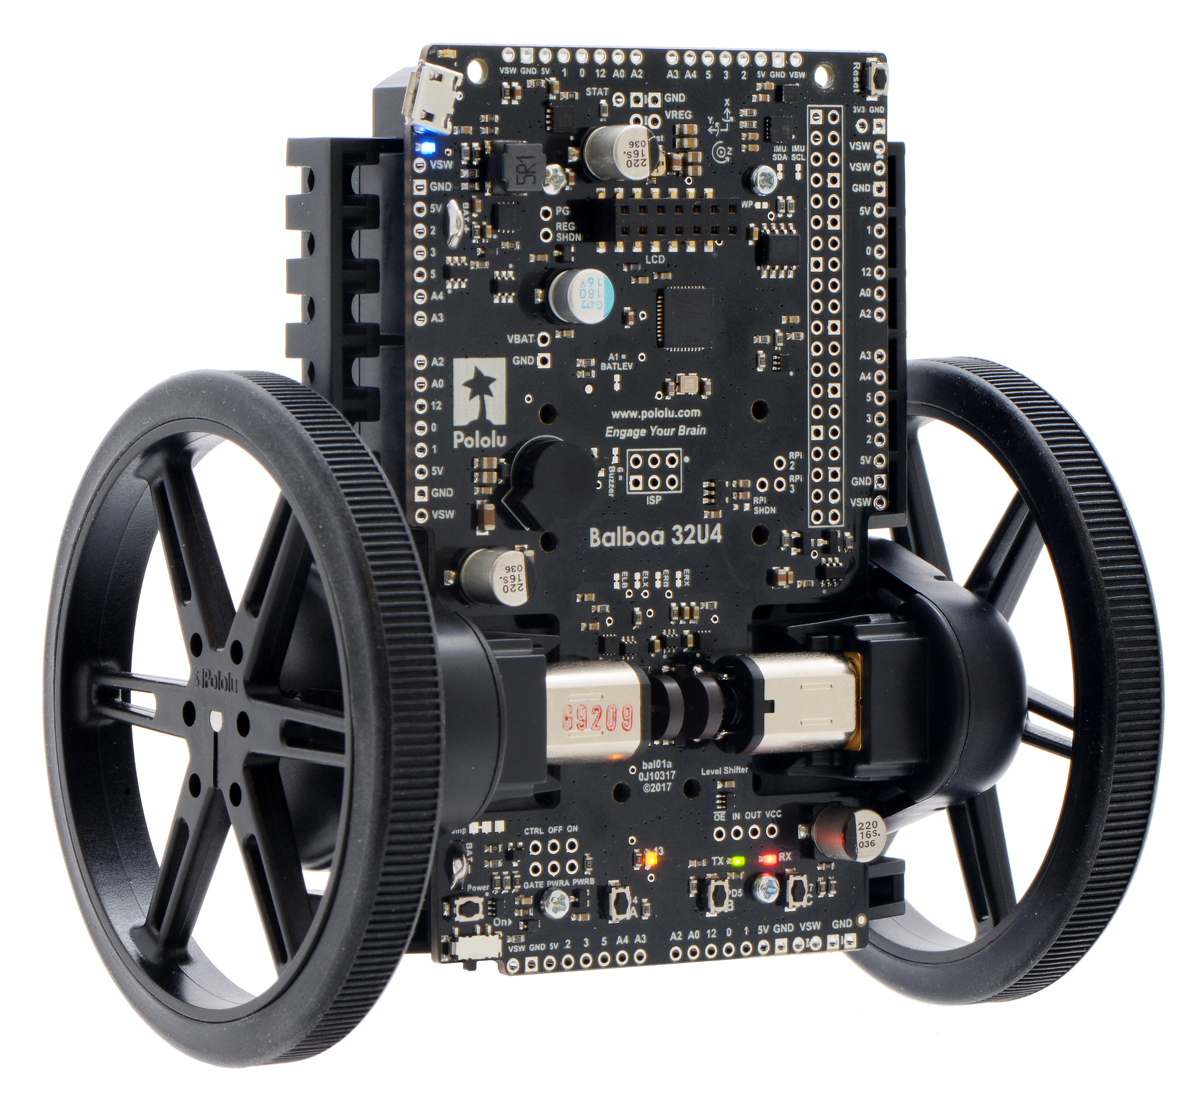
\includegraphics[width=0.55\linewidth]{robot3.jpg}
    \label{robot3}
\end{figure}

In order to begin working on our project, we first had to assemble the robot which was easily done in the following few steps:

\begin{enumerate}
    \item Install battery pack - Fig.\ref{robot0} 
    \item Solder motors - Fig.\ref{robot1}
    \item Assemble gears
    \item Attach wheels - Fig.\ref{robot2}
\end{enumerate}

\begin{figure}[H]
    \caption{Robot Assmebly Process}
    \begin{subfigure}{0.49 \textwidth}
        \centering
        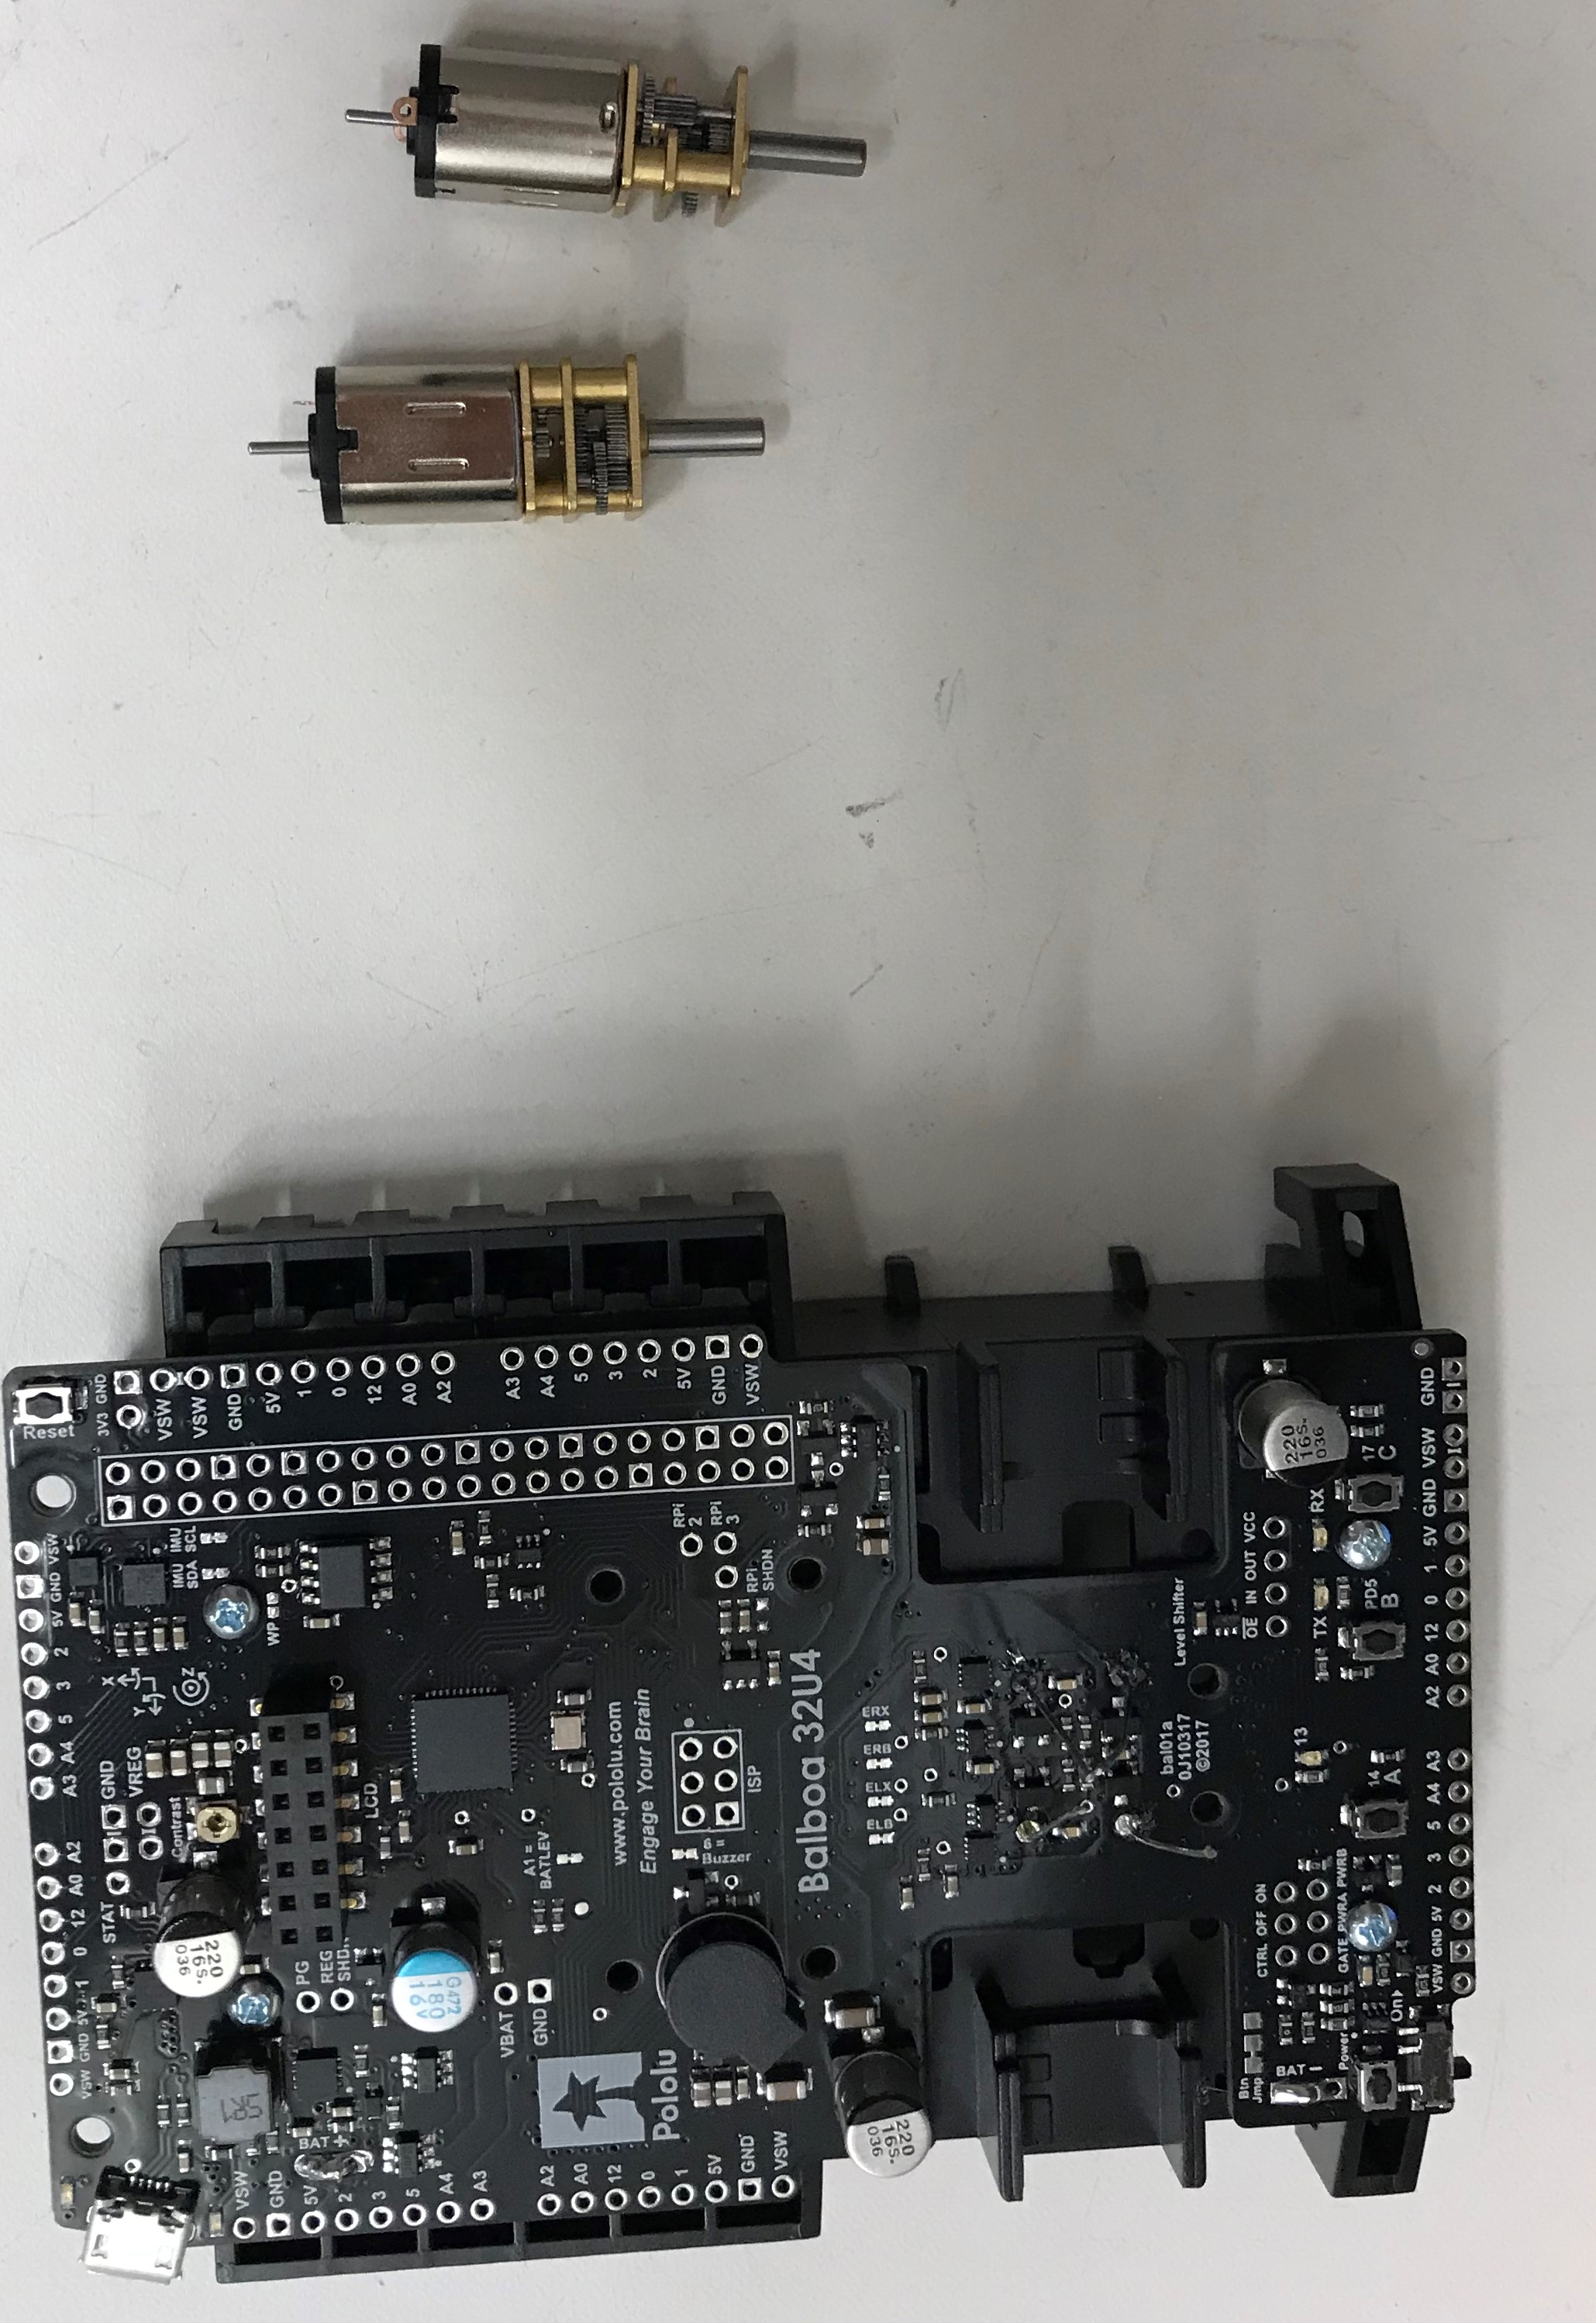
\includegraphics[width=0.7\linewidth]{robot0.jpg}
        \caption{Battery Pack Attached}
        \label{robot0}
    \end{subfigure}
    \begin{subfigure}{0.49 \textwidth}
        \centering
        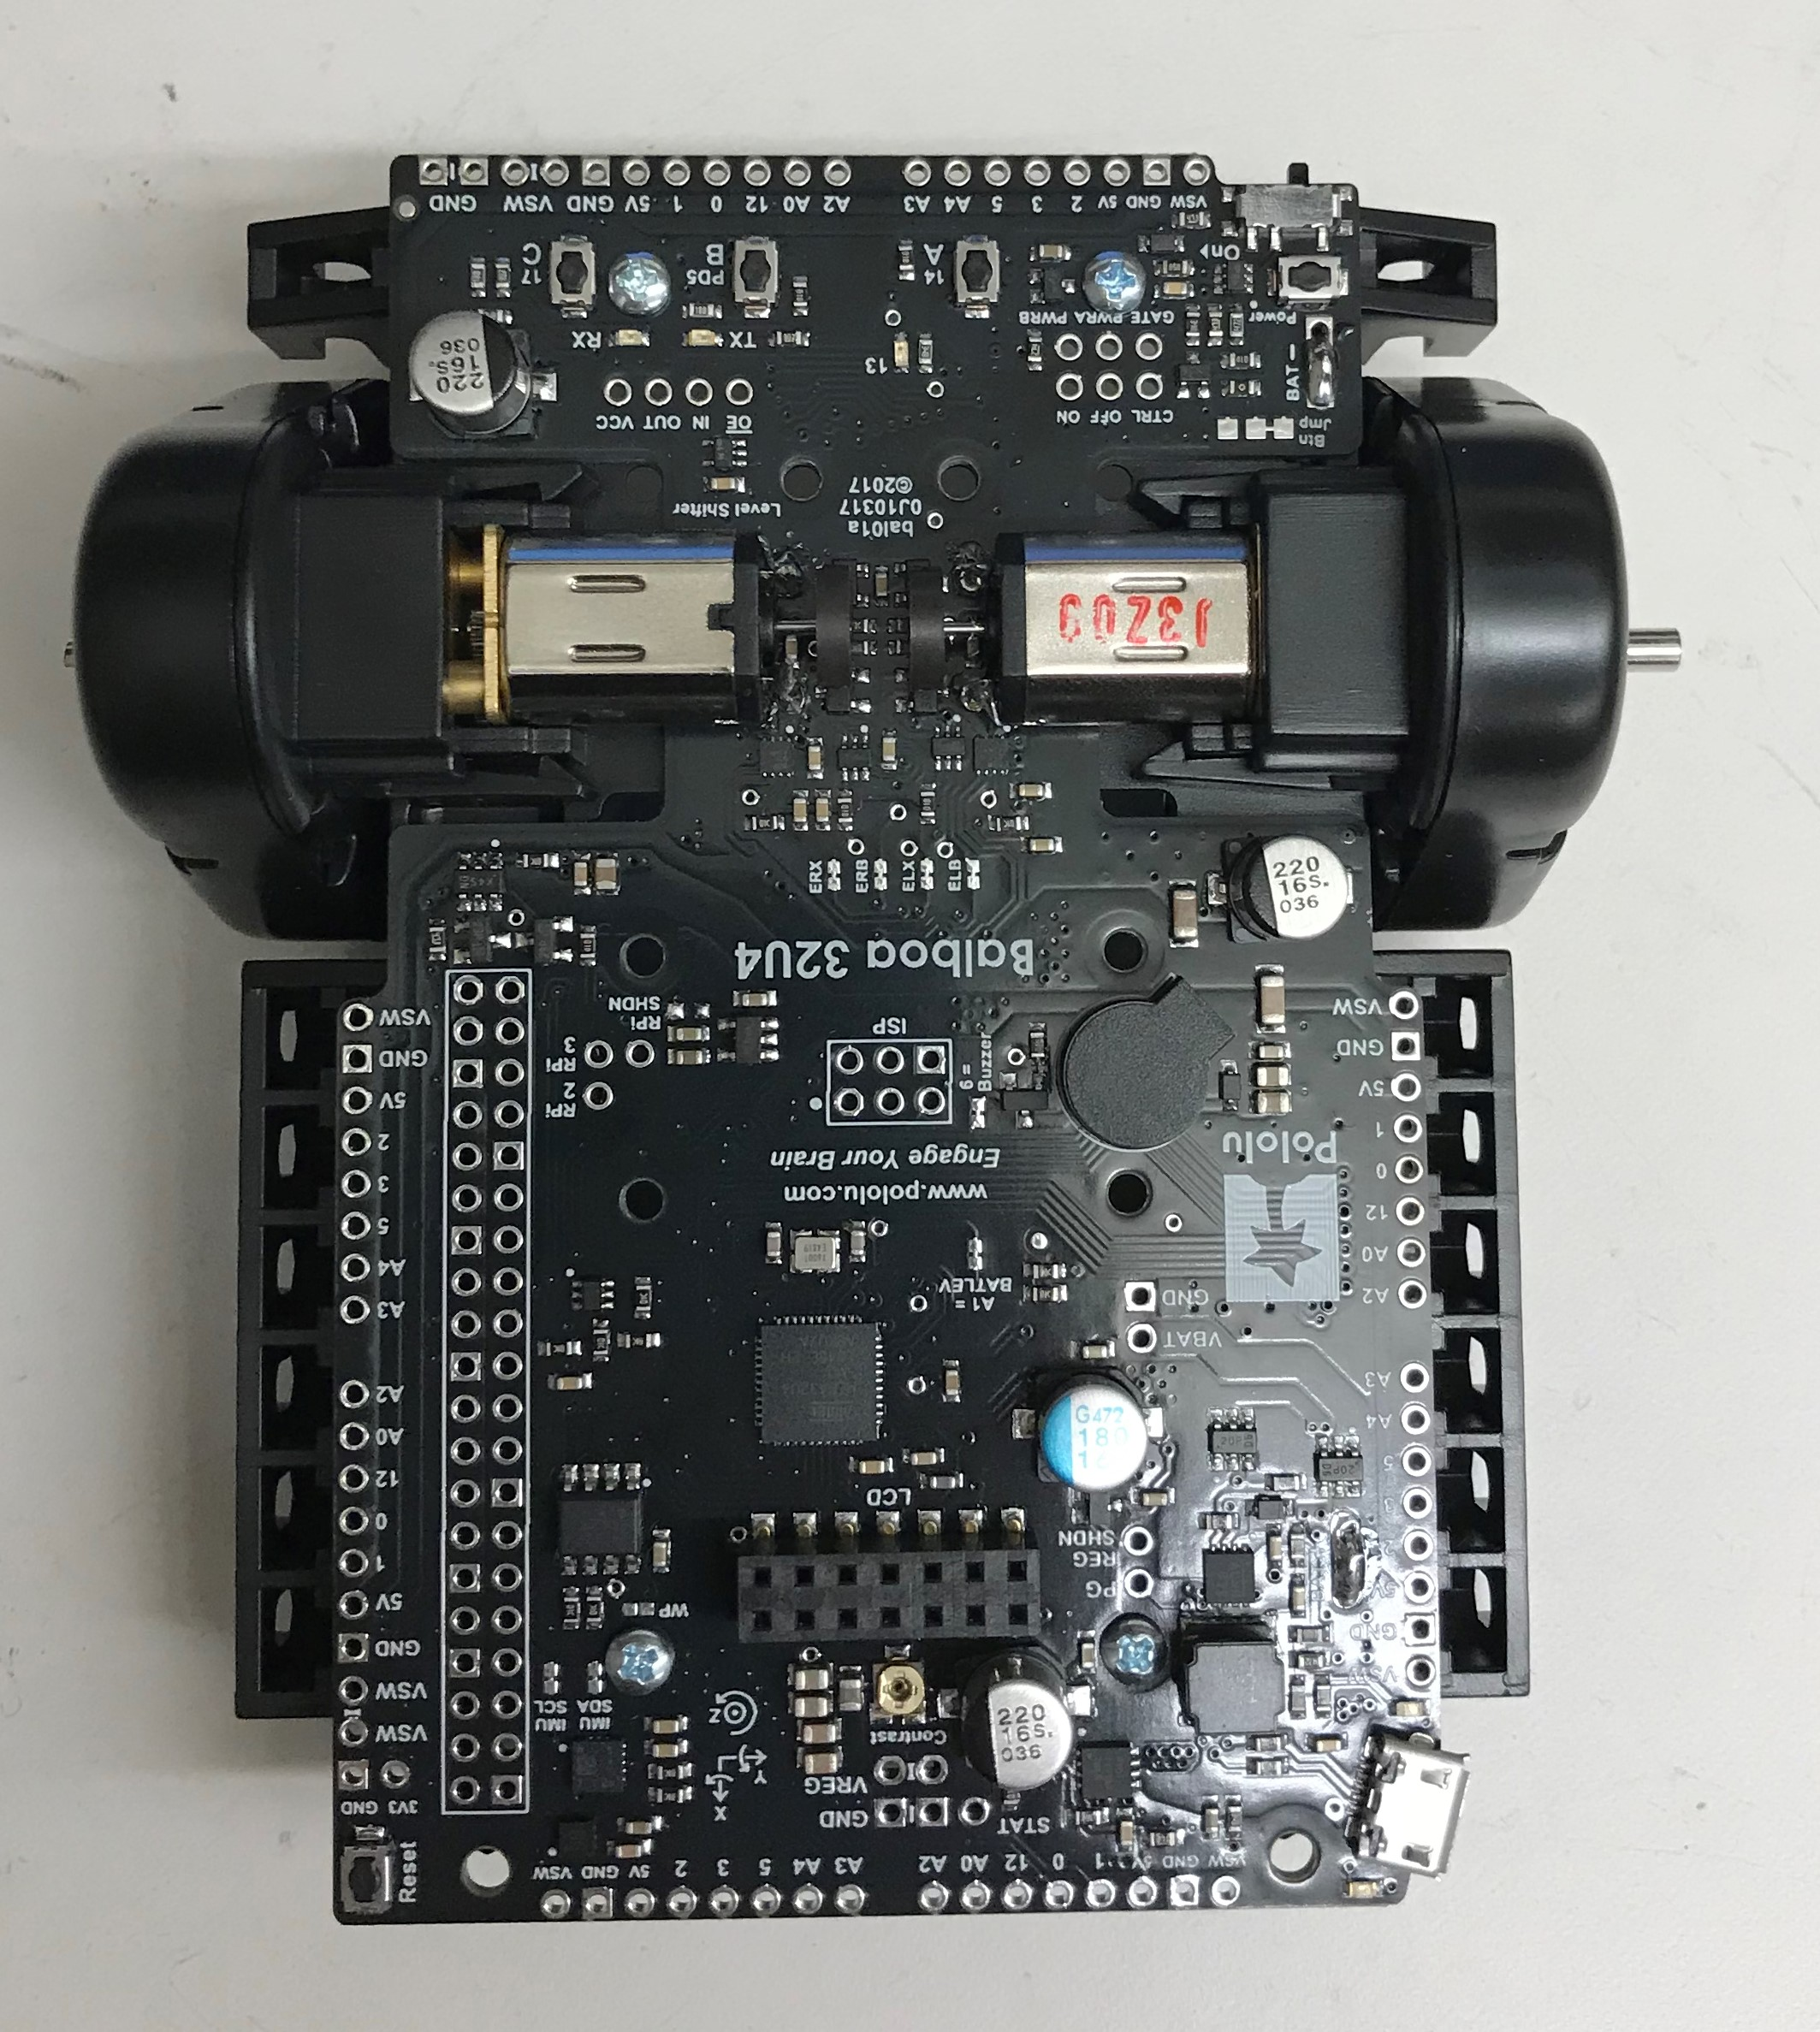
\includegraphics[width=0.9\linewidth]{robot1.jpg}
        \caption{Motors Soldered}
        \label{robot1}
    \end{subfigure}
    
    \begin{subfigure}{0.99 \textwidth}
        \centering
        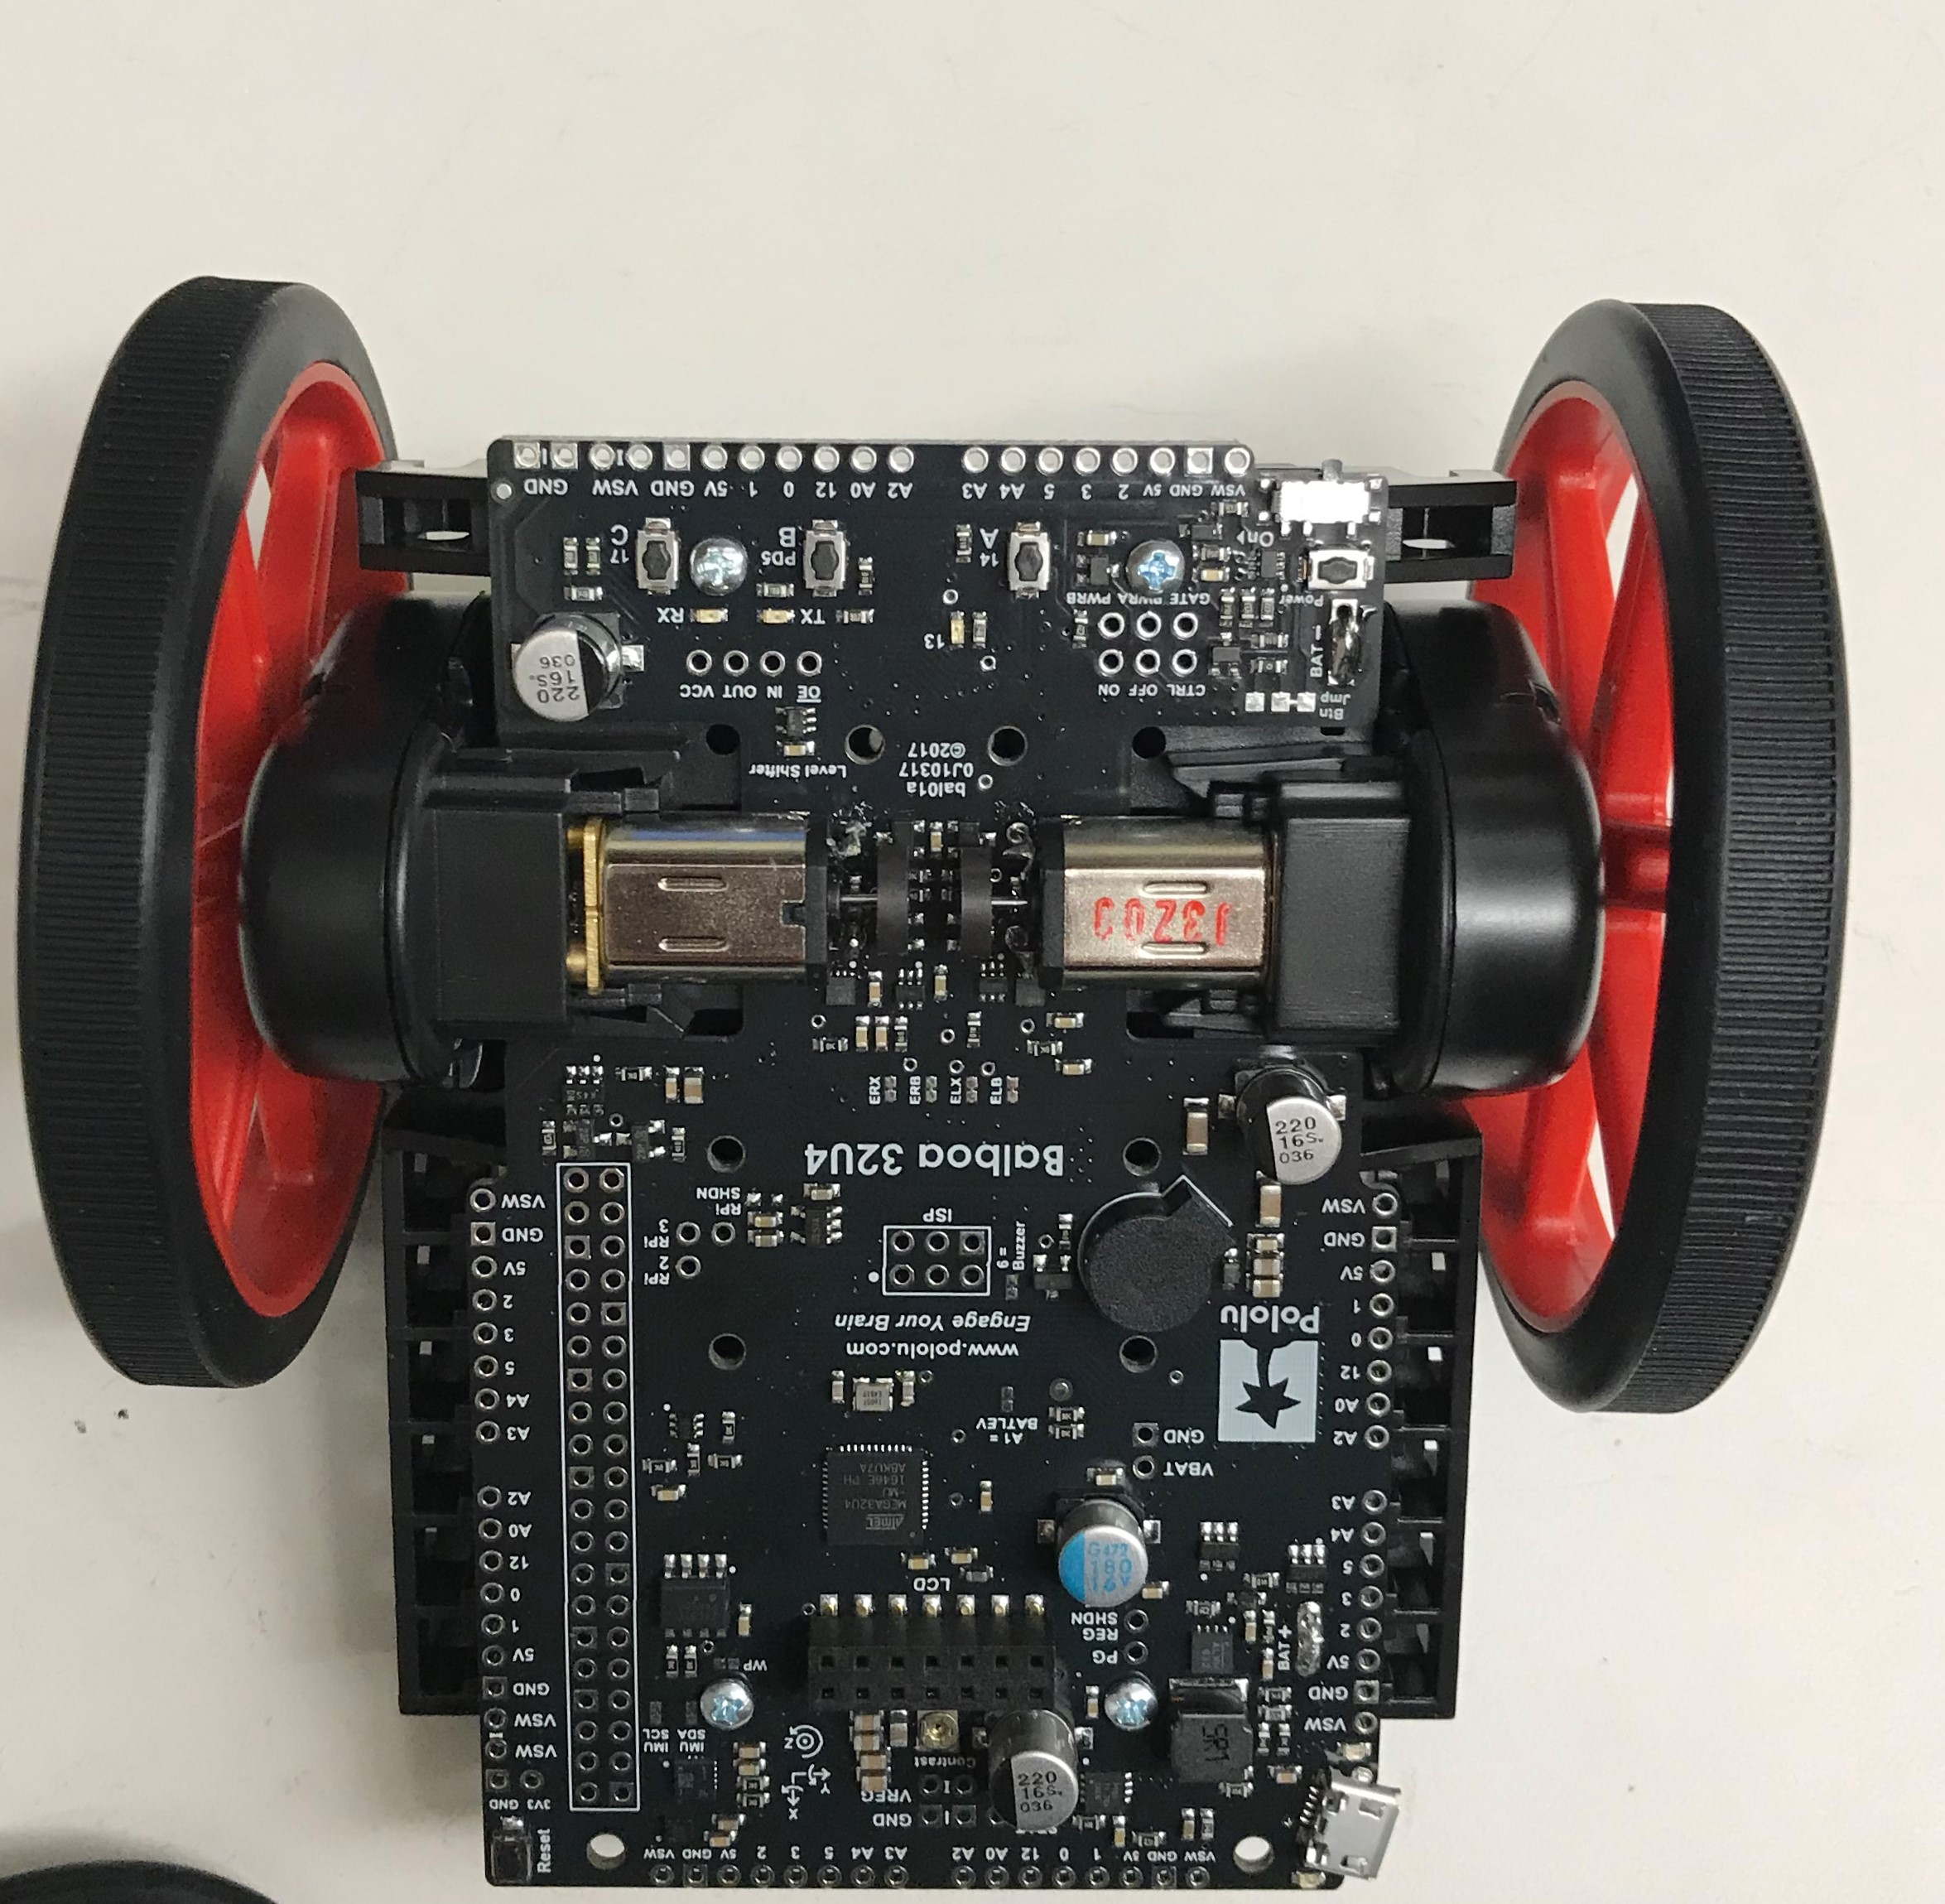
\includegraphics[width=0.45\linewidth]{robot2.jpg}
        \caption{Wheels Attached}
        \label{robot2}
    \end{subfigure}
\end{figure}

Furthermore, once assembling the robot, we made all the measurements necessary in order to model our system. The measurements are summarized in table \ref{motorMeas}.

\begin{table}[H]
    \centering
    \begin{tabular}{| c | c | c |}
        \hline   
        Symbol & Quantity & Measurement \\
        \hline
        $M_p$ & Mass of the robot & 0.2633\\
        $I_p$ & Moment of inertia of robot & 0.000325 \\
        $l$ & Half length & 0.02      \\
        $M_w$ & Wheel mass & 0.0198 \\
        $k_m$ & Motor torque constant & 3.0396\\
        $k_e$ & Motor back EMF constant & 0.3183 \\
        $R$ & Resistance & 20 \\
        $r$ & Wheel radius & 0.04 \\
        \hline
    \end{tabular}
    \caption{Motor Measurements}
    \label{motorMeas}
\end{table}

\vspace{5mm}
\section{State Space Model}

After assembling the robot and taking the measurements, we proceeded with the model development in order to find gains for the robot. The states we used are: $\theta$, the angle of the robot as shown above, $\dot \theta$, the angular velocity $x$, the distance and the velocity $\dot x$. 
First, we define the following variables:

\begin{align*}
    \beta &= 2*M_w + \frac{2I_w}{r^2} + M_p \\
    \alpha &= I_p\beta + 2M_pl^2(M_w+\frac{I_w}{r^2})
\end{align*}

With those variables, our state space model will have the following matrices:

\begin{align*}
    A &= 
    \begin{bmatrix}
        0 & 1 & 0 & 0 \\
        0 & \frac{2k_m k_e (Mp l r - I_p- M_p l^2)}{R \alpha r^2} & \frac{g M_p^2l^2}{\alpha} & 0\\
        0 & 0 & 0 & 1 \\
        0 & \frac{2k_m k_e(r \beta M_pl)}{(R \alpha r^2)} & \frac{M_p g l \beta}{\alpha} & 0 
    \end{bmatrix}\\
    B &= \begin{bmatrix}
        0 \\
        \frac{2k_m (I_p+M_p l^2 - M_p l r}{R r \alpha} \\
        0 \\
        \frac{2k_m (M_p l-r \beta )}{R r \alpha} 
    \end{bmatrix}\\
    E &= \begin{bmatrix}
        1 & 0 &-l &0 \\
        0 &1 &0 &-l\\
        0 &0 &1 &0 \\
        0 &0 &0 &1
    \end{bmatrix}
\end{align*}


Thus the model can be described with the following equation:
\[
    \frac{d}{dt}
    \begin{bmatrix}
        x \\
        \dot{x} \\
        \theta \\
        \dot{\theta}
    \end{bmatrix}
    =
    \begin{bmatrix}
        0 & 1 & 0 & 0 \\
        0 & \frac{2k_m k_e (Mp l r - I_p- M_p l^2)}{R \alpha r^2} & \frac{g M_p^2l^2}{\alpha} & 0\\
        0 & 0 & 0 & 1 \\
        0 & \frac{2k_m k_e(r \beta M_pl)}{(R \alpha r^2)} & \frac{M_p g l \beta}{\alpha} & 0 
    \end{bmatrix}
    \begin{bmatrix}
        x \\
        \dot{x} \\
        \theta \\
        \dot{\theta}
    \end{bmatrix}
    +
    \begin{bmatrix}
        0 \\
        \frac{2k_m (I_p+M_p l^2 - M_p l r}{R r \alpha} \\
        0 \\
        \frac{2k_m (M_p l-r \beta )}{R r \alpha} 
    \end{bmatrix}
    V
\]

\vspace{5mm}
\section{First Implementation}

For our first implementation, we used the LQR solver from \texttt{MATLAB} in the following way:
\begin{minted}{matlab}
    K = lqr(inv(Em)*Am,inv(Em)*Bm,Qp,Rp)
\end{minted}

The values of Qp and Rp we used are:
\begin{align*}
    Q_p &= \begin{bmatrix}
        0.025&0&0&0\\
        0&0.01&0&0\\
        0&0&1000&0 \\
        0&0&0&0.6
    \end{bmatrix}\\
    R_p &= 1    
\end{align*}

The resulting output was:
\[
K = \begin{bmatrix}
    0.15\\
    0.1\\
    32\\
    0.8
\end{bmatrix}    
\]

\begin{figure}[H]
    \caption{Initial LQR output}
    \centering
    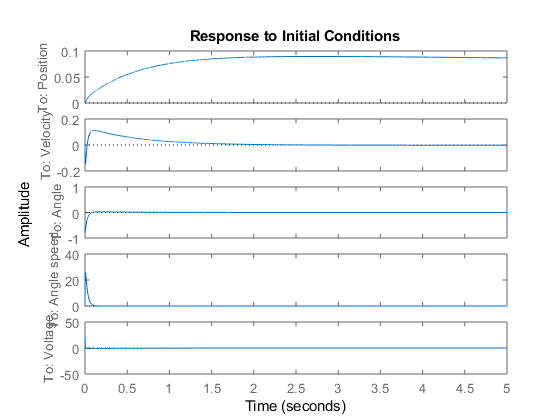
\includegraphics[width=0.6\textwidth]{lqrOut_initial.png}
    \label{lqr1}
\end{figure}


Even though the system was not predicted to be entirely stable, (Fig.\ref{lqr1}) we decided to try it. The robot managed to stay stable for a few seconds, but would quickly start oscillating wildly and get out of control. We first tried implementing a digital filter ($V[t] = 0.9V[t] + 0.1V[t-1]$) in order to reduce the "jitter", but that barely helped.

As seen in Fig. \ref{robot_bad}, the robot was unable to return to a stable position. Furthermore, what is interesting in the data is how often we reach the maximum voltage of 5V. From this it was obvious that we had to reduce our gains.

\begin{figure}[H]
    \caption{Initial Gains Real System Response}
    \centering
    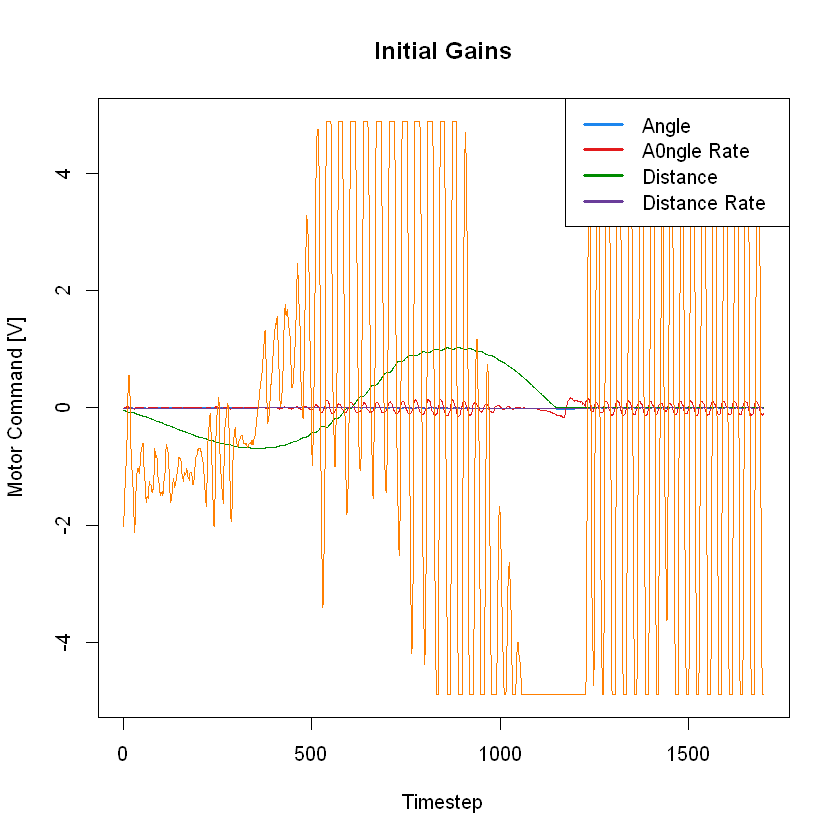
\includegraphics[width=0.7\textwidth]{initialGains.png}
    \label{robot_bad}
\end{figure}

\section{Final Implementation}

In order to make our robot more stable, we decreased the angle gain, and increased the velocity gain, such that our gain matrix was. Performing LQR again with:

\begin{align*}
    Q_p &= \begin{bmatrix}
        0.25&0&0&0\\
        0&170&0&0\\
        0&0&740&0 \\
        0&0&0&0.05
    \end{bmatrix}\\
    R_p &= 1    
\end{align*}

And taking into account the rotation of our motors, we get:
\[
\begin{bmatrix}
    0.5 \\
    7.5\\
    28\\
    0.3    
\end{bmatrix}    
\]

The predicted response according to \texttt{MATLAB} seemed good \ref{lqrf}.

\begin{figure}[H]
    \caption{Initial LQR output}
    \centering
    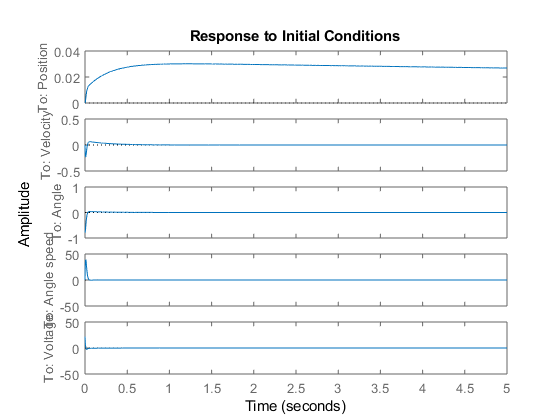
\includegraphics[width=0.6\textwidth]{lqrOut_final.png}
    \label{lqrf}
\end{figure}

Additionally, in order to reduce the jitter, not only did we keep the digital filter, but we also slightly increased our timestep size.

The final robot was able to stand for an indefinite amount of time without much oscillation and was able to recover to stability after external disturbances, as is obvious in figure \ref{goodRobot}.

\begin{figure}[H]
    \caption{Initial Gains Real System Response}
    \centering
    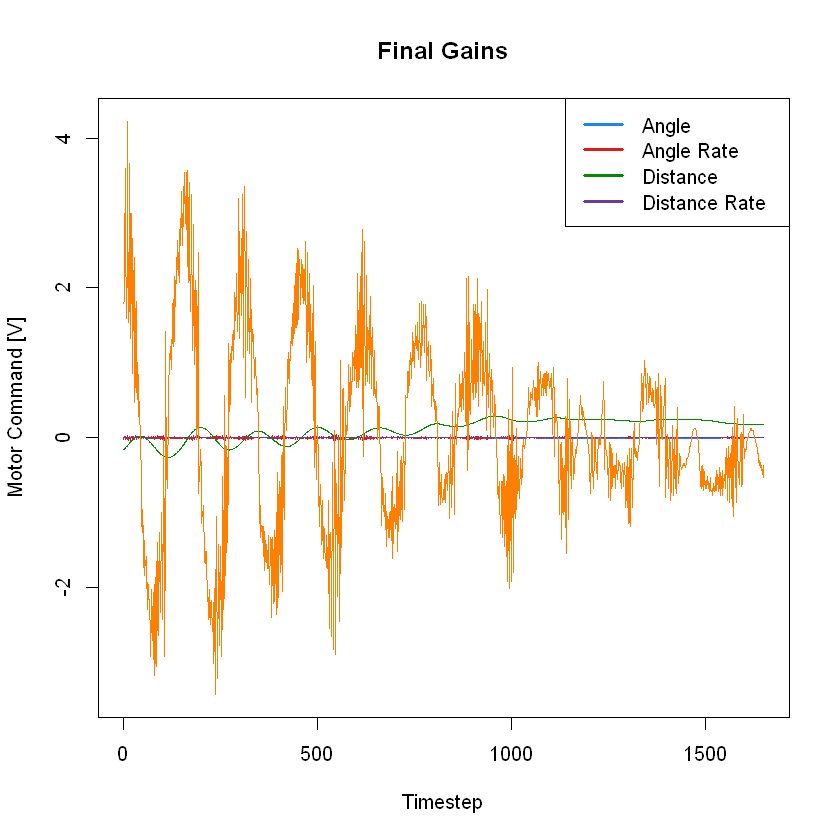
\includegraphics[width=0.8\textwidth]{finalGains.png}
    \label{goodRobot}
\end{figure}

\section {Conclusion}
The inverted pendulum is a very interesting problem in control theory. We attempted to solve it using LQR and we reached a relatively good result. More detailed measurements and accurate motor data, could provide the missing information for an even more stable system. It would also be interesting to see how the system identification method would work for this sort of problem.

\end{document}